\section{The algorithm}
In 1972 and 1974, the National Bureau of Standards (now the National Institute of Standards and Technology, or NIST) issued the first public request for an encryption standard. The result was DES\cite{NBS77}, which became widely used and a very successful encryption algorithm at the time. However, due to advances in distributed key search techniques, the key was found to be too short for modern security applications.
Triple-DES emerged as a temporary solution in many high-security applications, such as banking, but was too slow. More fundamentally, the $64$-bit block length shared by DES and most other well-known ciphers opens it up to attacks when large amounts of data are encrypted under the same key.

Twenty years later, in 1997, NIST announced the Advanced Encryption Standard (AES)\cite{NIST97a}. NIST requested comments from the public on the proposed standard, and eventually issued a call for algorithms to satisfy the standard\cite{NIST97b}. NIST made all submissions public and eventually, through a process of public review and comment, chose a new encryption standard to replace DES. Twofish did not win, but made it as one of the five finalists in the 1997 competition.

Figure~\ref{fig:twofish} shows the Twofish algorithm. It is a $16$ byte / $128$-bit block cipher with a variable key length between $128$ and $256$ bits.
The cipher is a $16$-round Feistel network also called a substitute-permute network. It has a bijective function $F$ consisting of four key-dependent $8$-by-$8$-bit S-boxes (Substitution-boxes)\cite{wiki_sbox}, a fixed $4$-by-$4$ MDS (maximum distance separable) matrix over GF($2^8$) (Galois-field), a PHT (pseudo-Hadamard transform), bitwise rotations, and a carefully designed key schedule.
\begin{figure}[tp]
  \centering
  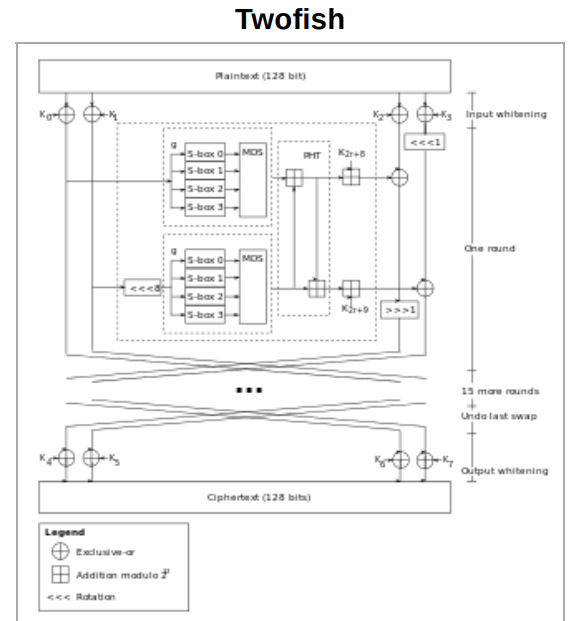
\includegraphics[scale=0.4]{Graphics/twofish.png}
  \caption{The Twofish algorithm}
  \label{fig:twofish}
\end{figure}

\subsection{Feistel Networks}
A Feistel network is a general method of transforming any function (usually called the F function) into a permutation. It was invented by Horst Feistel in 1973.

The fundamental building block of a Feistel network is the $F$ function: a key-dependent mapping of an input string onto an output string. An $F$ function is always non-linear and possibly non-surjective\footnote{A non-surjective F function is one in which not all outputs in the output space can occur.}:

\begin{equation*}
  F : \lbrace 0, 1\rbrace^{n/2} x \lbrace0, 1\rbrace^N -> \lbrace 0, 1\rbrace^{n/2}
\end{equation*}

where $n$ is the block size of the Feistel network, and $F$ is a function taking $n/2$ bits of the block and $N$ bits of a key as input, and producing an output of length $n/2$ bits.
In each round, the ``source block`` is the input to $F$ , and the output of $F$ is XOR'ed with the ``target block``, after which these two blocks swap places for the next round.
The idea here is to take an $F$ function, which may be a weak encryption algorithm when taken by itself, and repeatedly iterate it to create a strong encryption algorithm.
Two rounds of a Feistel network is called a \emph{cycle}.
In one cycle, every bit of the text block has been modified once.

This is in fact very similar to what happens in \emph{discrete wavelet transformation} (DWT), where the technique called a \emph{lifting scheme} was introduced by Wim Sweldens.

\subsection{S-boxes}
An S-box is a table-driven non-linear substitution operation used in most block ciphers.
S-boxes vary in both input size and output size, and can be created either randomly or algorithmically.
S-boxes were first used in Lucifer by Horst Feistel, then DES, and afterwards in most encryption algorithms.
Twofish uses four different, bijective, key-dependent, $8$-by-$8$-bit S-boxes.
These S-boxes are built using two fixed $8$-by-$8$-bit permutations and key material.

\subsection{A small 2-by-2-bit S-box example}
Substitute-permute networks, as the name implies, perform a substitution followed by a permutation.
Two bits can have four different values: ``00``, ``01``, ``10`` and ``11``, so a table could look like this:
\begin{table}[htp]
  \begin{center}
    \label{fig:small_subs_example}
    \begin{tabular}{|l|c|c|c|c|}
      \hline
      input  & 00 & 01 & 10 & 11 \\ \hline
      output & 10 & 00 & 11 & 01 \\ \hline
    \end{tabular}
  \end{center}
\end{table}

If ``10`` enters the table, it becomes substituted to ``11`` and if ``11`` enters it becomes substituted to ``01``.
Given two of these $2$-by-$2$-bit S-boxes, the output would be 2 bits from each, equalling $4$ in total.
The permutation part is switching bits and could look like this:
\begin{table}[htp]
  \begin{center}
    \label{fig:small_permu_example}
    \begin{tabular}{|l|c|c|c|c|c|c|c|c|}
      \hline
      input  & 0  & 1  & 2  & 3  & 4  & 5  & 6  & 7  \\ \hline
      output & 6  & 13 & 15 & 1  & 7  & 12 & 8  & 3  \\ \hline
      input  & 8  & 9  & 10 & 11 & 12 & 13 & 14 & 15 \\ \hline
      output & 2  & 0  & 14 & 10 & 5  & 9  & 11 & 4  \\ \hline
    \end{tabular}
  \end{center}
\end{table}

Given input ``0100``, the first Sbox would have input ``01`` and the second Sbox to have input ``00``.
The output of the first S-box equals ``00`` and the output of the second S-box equals ``10``.
So in decimal, the number $4$ goes through the two S-boxes and comes out as a $2$.
Then it enters the permutation table and becomes $15$ constituting one round of substituting and permuting.
This process is very easy to reverse if the substition table and the permutation table are public, hence Twofish mixes in keys via XOR.
It XORs before the first encryption (input whitening), after each round, and again after the last round (output whitening).
Without the key, the process becomes very hard to reverse.
There is a trade-off of security versus speed; too few rounds makes the encryption breakable whereas too many rounds will make it slow.
Twofish uses $16$ rounds compared to the $10-14$ for AES depending on key size.

\subsection{Maximum Distance Seperable matrices}
An MDS matrix is a linear mapping from $a$ field elements to $b$ field elements. It produces a composite vector of $a + b$ elements with the property that for each non-zero vector there will be atleast $b + 1$ non-zero elements.
What this means is that the ``distance`` (i.e. the number of elements that differ) between two distinct vectors produced by the MDS mapping is atleast $b + 1$.
It is provable that no mapping can have a larger minimum distance between two distinct vectors\cite{TwofishPaper}, hence we call it Maximum Distance Seperable.
Twofish uses a $4$-by-$4$ MDS matrix over GF ($2^8$) called the Reed-Solomon (RS) error-correcting codes.

\subsection{Pseudo-Hadamard transforms}
The $32$-bit pseudo-Hadamard transform (PHT) that Twofish uses is a mixing operation that given two inputs $a$ and $b$, updates the two values as follows:
\begin{equation*}
  a' = a + b\text{ mod }2^{32} \\
\end{equation*}
\begin{equation*}
  b' = a + 2b\text{ mod }2^{32}
\end{equation*}
This is used to mix the two outputs of its \emph{g} function calls.

\subsection{Whitening}
Input/output whitening is done by XOR'ing $128$ bits of subkey, which is not used in any of the rounds, with part of the expanded key before the first round and after the last round. It was shown in 1996 by Rivest\cite{KR96} that whitening made it substantially harder for attackers to do keysearch attacks.

\subsection{Key schedule}
\label{section:key_schedule}
The key schedule is the means by which the key bits are turned into round keys that the cipher can use.  Twofish needs a lot of key material, and has a complicated key schedule. To facilitate analysis, the key schedule uses the same primitives as the round function.

There are two types of keys used for the Twofish algorithm.
It uses a user-supplied global key $M$ of $128$ bits to generate two sets of subkeys $S$ and $K$.
$S$ has two subkeys $S_0$ and $S_1$ which are fixed during the entire encryption and decryption process.
$S_0$ and $S_1$ are used in the S-boxes inside the g function.
The key schedule performs a key expansion to make K, which is a $40$-word expanded key where each word consists of $32$ bits.
$K_0$-$K_7$ are used for input / output whitening whilst the remaining $32$ words are passed to the bijective function F two at a time during the 16 rounds of encryption.
$S$ is generated by finite field multiplication in Galois Field GF$(2^8)$ where the primitive polynomial is $x^8 + x^6 + x^3 + x^2 + 1$.
Finite field multiplication would be implemented in Hermes using Bennett embedding, as the multiplication can sometimes have values that are zero.
Bennett embedding would allow us to save the values until decomputed later.
